\documentclass[10pt]{article}

% Workshop-preprint formatting (self-contained, no venue style file required).
% To submit, swap the preamble for the venue's official style (e.g. neurips_2026.sty
% with the workshop option) — the body is written to drop in unchanged.
\usepackage[margin=1in]{geometry}
\usepackage{newtxtext,newtxmath}
\usepackage{graphicx}
\usepackage{booktabs}
\usepackage{multirow}
\usepackage{amsmath}
\usepackage{braket}
\usepackage{microtype}
\usepackage[numbers,sort&compress]{natbib}
\usepackage[colorlinks=true,linkcolor=blue,citecolor=blue,urlcolor=blue]{hyperref}
\usepackage{caption}
\captionsetup{font=small,labelfont=bf}

\title{\bf When Does a Variational Quantum Classifier Head Help?\\
\large An Empirical Comparison Against Near-Parameter-Matched Classical Heads\\
on MNIST and CIFAR-10}

\author{%
  Alexander Greene\\
  \texttt{alexanderngreene@gmail.com}\\
}

\date{}

\begin{document}
\maketitle

\begin{abstract}
Hybrid image classifiers that feed a convolutional network into a small
variational quantum circuit (VQC) are a common near-term quantum machine
learning design, but reported gains are hard to interpret without matched
baselines and matched tuning. We train a shared CNN backbone with an
8-dimensional bottleneck and three interchangeable heads (a linear layer, a
near-parameter-matched MLP, and an 8-qubit VQC) on low-data subsets of MNIST
and CIFAR-10. An exploratory sweep with one shared training recipe suggested a
large VQC advantage over the MLP on MNIST (7--18 points) and a large VQC
deficit on CIFAR-10 (8--14 points). We re-ran the comparison with longer
training, a train/validation/test split and the same validation-based
learning-rate search for every head. The mean MNIST advantage shrinks to at
most about 3 points (paired over seeds), and the CIFAR-10 deficit to 9.2, 8.9 and
3.1 points at 1{,}000, 2{,}000 and 4{,}000 samples. A linear head has the highest mean
accuracy in every condition. We then trained every head on identical frozen
embeddings. On embeddings from VQC-trained backbones, a linear readout beats
the VQC by 1.6--1.7 points, consistently across seeds. On embeddings from
linear-trained backbones, whose values mostly saturate the $\pi\tanh$ angle
encoding, the VQC collapses, and so, largely, does a classical Fourier-feature
head with the same encoding. Fixed input standardization recovers most of the
loss, a learned rescaling recovers a little more, and one tripled training
budget recovers little. In this bounded study, the VQC head's behavior tracks
classical factors (the training recipe, and the match between the embedding
distribution and the encoding), and in no selected configuration does it
outperform a linear readout.
\end{abstract}

\section{Introduction}

Variational quantum circuits (VQCs) trained by gradient descent are the
workhorse of near-term quantum machine learning
\citep{benedetti2019parameterized, cerezo2021variational}. In image
classification, a common hybrid pattern delegates feature extraction to a
classical convolutional network and classification to a small quantum circuit
\citep{mitarai2018quantum, havlicek2019supervised}. Reported successes are
difficult to interpret: quantum heads are frequently compared against classical
baselines with different parameter budgets, different backbones, untuned
hyperparameters, or no seed replication. Bowles et al.\ \citep{bowles2024better}
benchmarked 12 quantum models on 160 datasets and found that simple classical
baselines generally match or beat them, and that removing entanglement often
does not hurt. Their models read fixed, low-dimensional inputs. We study the
image-classification pattern, where a CNN is trained \emph{through} the circuit,
and ask how much of a head comparison reflects the head itself, the backbone it
induces, and the training recipe.

Our question is narrow: \emph{holding the backbone architecture, the bottleneck
dimension and the optimizer fixed, and matching head parameter counts as
closely as the architectures allow, does replacing a classical classifier head
with a VQC help?} We contribute:

\begin{enumerate}
  \item An exploratory comparison of linear, near-parameter-matched MLP, and
        VQC heads (with three data re-uploading schedules) under one shared
        training recipe on MNIST and CIFAR-10: 90 reported runs, plus two
        documented unreported CIFAR-10 sweeps (Section~\ref{sec:results}).
  \item A re-run of the head comparison under a train/validation/test protocol
        with an equal learning-rate search for every head (297 runs,
        Section~\ref{sec:protocol}). Most of the head differences in the
        exploratory sweep, in both directions, turn out to depend on the
        shared training recipe: on MNIST largely on its short epoch budget and
        protocol, on CIFAR-10 largely on its learning rate.
  \item A frozen-embedding experiment (498 head fits,
        Section~\ref{sec:frozen}) that separates the head from the backbone
        it induces. It compares fixed and learned input rescaling with a
        longer training budget, and includes a classical control that shares
        the VQC's input encoding.
\end{enumerate}
The negative result is the main finding: in this setting we find no condition
in which the VQC head beats a linear readout, and its large apparent advantage
over an MLP shrinks to a few points under matched tuning.

\section{Architecture and Methods}
\label{sec:methods}

\paragraph{Shared backbone.}
All heads use the same backbone architecture and embedding dimension: a CNN
backbone ends in global average pooling followed by a linear projection to a
$d=8$ dimensional bottleneck. Each head is trained jointly with its own copy of
the backbone, so the embeddings themselves differ (Section~\ref{sec:frozen}). For
MNIST the backbone has three convolutional blocks (32--64--128 channels,
${\sim}94$K parameters); for CIFAR-10, four blocks (64--128--256--256
channels, ${\sim}0.96$M parameters). The backbone is trained jointly with the
head in every run; gradients flow through the quantum circuit into the
convolutional layers.

\paragraph{Quantum head.}
The bottleneck vector $\mathbf{x} \in \mathbb{R}^8$ is encoded into an 8-qubit
circuit by single-qubit rotations $R_y\!\left(\pi \tanh x_i\right)$ on qubit
$i$. The variational block repeats $L=4$ layers, each applying learned
$R_y(\theta)\,R_z(\phi)$ rotations per qubit followed by a ring of CNOT
entanglers. The circuit outputs $\braket{Z_i}$ for each qubit, and a final
classical linear layer maps the 8 expectation values to 10 class logits. The
head stores 154 trainable parameters: $8 \times 2 \times 4 = 64$ rotation
angles plus $8 \times 10 + 10 = 90$ readout weights. Only 146 of them can
affect the output. The last layer's eight $R_z$ rotations only change the
phases of computational-basis amplitudes; what follows them is a CNOT ring,
which permutes basis states, and $Z$ measurements, which depend only on
amplitude magnitudes. Those phases therefore never reach any $\braket{Z_i}$. Parameter counts are used here only to
size the baselines; they are not a measure of capacity. Rotation angles are
initialized from $\mathcal{U}(-0.1, 0.1)$, which starts every rotation gate
near the identity (the CNOT ring is unaffected), instead of PennyLane's default $\mathcal{U}(0, 2\pi)$; in
preliminary runs the default produced much larger seed-to-seed variance.
In the exploratory sweep, circuits are simulated with PennyLane's
\texttt{lightning.qubit} statevector backend using adjoint differentiation
\citep{bergholm2018pennylane}. Sections~\ref{sec:protocol}--\ref{sec:frozen}
use a batched PyTorch statevector simulator of the same circuit, which matches
PennyLane to $10^{-6}$ in outputs and in input and weight gradients.

\paragraph{Data re-uploading.}
We test three encoding schedules. \textsc{none} encodes $\mathbf{x}$ once,
before the first variational layer. \textsc{light} additionally re-encodes a
rescaled copy ($0.5\mathbf{x}$) midway through the variational block.
\textsc{strong} places one full encoding of $\mathbf{x}$ immediately before
\emph{each} of the $L=4$ variational layers (the first of these serves as the
initial encoding; there is no separate extra encoding), following
P\'{e}rez-Salinas et al.~\citep{perez2020data}.

\paragraph{Classical baselines.}
The \emph{linear} head is a single dense layer (90 parameters). The \emph{MLP}
head is $8 \to 8 \to 10$: one hidden layer of width 8 with ReLU activation, no
dropout or normalization, PyTorch-default (Kaiming-uniform) initialization,
and, in the exploratory sweep, the same optimizer and learning rate as every
other head (Section~\ref{sec:protocol} tunes each head separately). Its 162 total parameters (weights and biases of both layers) are
the closest the architecture comes to the quantum head's 154; we therefore
describe the MLP as \emph{near}-parameter-matched rather than equal. The
linear head is smaller than both and is included as the strongest simple
reference baseline (a linear probe of the embedding), not as a
capacity-matched comparison.

\paragraph{Training recipe (exploratory sweep).}
All runs use AdamW (head learning rate $10^{-3}$, backbone $5\times10^{-4}$,
weight decay $10^{-4}$), cosine-annealed to zero over the run, batch size 32,
and gradient clipping. Training subsets are stratified samples of the full
training set, preserving class balance. MNIST runs train for 25 epochs with
clip norm 1.0; CIFAR-10 runs for 80 epochs with clip norm 2.0 and standard
augmentation (random crop, horizontal flip, rotation, color jitter). Every
configuration is repeated with seeds $\{0, 1, 2\}$; we report the mean and
\emph{sample} standard deviation over the three seeds. Per-component gradient
norms (backbone vs.\ head) are logged every epoch to monitor trainability.

\paragraph{Evaluation caveat.}
In the original sweeps (Tables~\ref{tab:mnist}--\ref{tab:cifar}), accuracy is
measured on the official 10{,}000-image test split after every epoch and we
report the best epoch per run, so the test split participates in checkpoint
selection; we call this metric \emph{test-split accuracy}. Mean final-epoch
accuracy is within 1.35 points of best-epoch accuracy in all 30
configurations (within 0.5 points in 19), and no ordering among heads changes
if final-epoch accuracy is used instead. That comparison does not bound the
bias from choices made while looking at these numbers (initialization,
augmentation, which sweep to report), so we treat Tables~\ref{tab:mnist}--%
\ref{tab:cifar} as exploratory and re-run the headline comparison under a
proper train/validation/test protocol in Section~\ref{sec:protocol}.

\paragraph{Sweep provenance.}
Table~\ref{tab:mnist} is the 25-epoch MNIST sweep; Table~\ref{tab:cifar} is the
last of three completed 80-epoch CIFAR-10 sweeps. The two unreported ones
differ as follows. One used weight
decay $10^{-3}$ instead of $10^{-4}$. The other has identical recorded settings
but, judging from its much larger logged train--test gaps, predates the
addition of random rotation and color jitter to the augmentation pipeline
(augmentation was not recorded in run metadata at the time, so this is an
inference). We report the most recent sweep because it reflects the final
pipeline. All three give the same ordering of heads at every size (linear $>$
MLP $>$ quantum \textsc{none} $>$ \textsc{light} $>$ \textsc{strong}); the
unreported weaker-augmentation sweep is \emph{more} favorable to the quantum
head (62.9\% vs.\ 58.9\% at 4{,}000 samples). Per-cell numbers for all three are
in the released logs.

\section{Exploratory Sweep: One Shared Recipe}
\label{sec:results}

\begin{table}[t]
\centering
\caption{Best test-split accuracy (\%, mean $\pm$ sample std over 3 seeds) on
stratified MNIST subsets. Bold marks the better of the two
near-parameter-matched heads (MLP vs.\ quantum).}
\label{tab:mnist}
\small
\begin{tabular}{lccccc}
\toprule
& & & \multicolumn{3}{c}{Quantum (re-uploading schedule)} \\
\cmidrule(lr){4-6}
Train size & Linear & MLP & \textsc{none} & \textsc{light} & \textsc{strong} \\
\midrule
250   & 61.5 $\pm$ 1.7 & 36.7 $\pm$ 5.4 & \textbf{54.5 $\pm$ 3.7} & 48.3 $\pm$ 10.7 & 38.3 $\pm$ 7.4 \\
500   & 79.3 $\pm$ 2.9 & 53.2 $\pm$ 6.9 & \textbf{71.2 $\pm$ 1.9} & 57.8 $\pm$ 2.5 & 45.6 $\pm$ 6.7 \\
1{,}000 & 89.6 $\pm$ 0.7 & 76.4 $\pm$ 3.4 & \textbf{83.3 $\pm$ 0.3} & 68.4 $\pm$ 3.5 & 54.6 $\pm$ 14.0 \\
\bottomrule
\end{tabular}
\end{table}

\begin{table}[t]
\centering
\caption{Best test-split accuracy (\%, mean $\pm$ sample std over 3 seeds) on
stratified CIFAR-10 subsets. Bold marks the better near-parameter-matched
head.}
\label{tab:cifar}
\small
\begin{tabular}{lccccc}
\toprule
& & & \multicolumn{3}{c}{Quantum (re-uploading schedule)} \\
\cmidrule(lr){4-6}
Train size & Linear & MLP & \textsc{none} & \textsc{light} & \textsc{strong} \\
\midrule
1{,}000 & 57.5 $\pm$ 0.8 & \textbf{51.2 $\pm$ 0.8} & 37.1 $\pm$ 2.4 & 34.2 $\pm$ 0.7 & 26.6 $\pm$ 1.9 \\
2{,}000 & 64.6 $\pm$ 0.7 & \textbf{60.6 $\pm$ 0.9} & 46.8 $\pm$ 5.2 & 42.7 $\pm$ 3.9 & 28.7 $\pm$ 1.9 \\
4{,}000 & 71.2 $\pm$ 0.5 & \textbf{67.2 $\pm$ 0.4} & 58.9 $\pm$ 4.6 & 52.0 $\pm$ 7.8 & 35.2 $\pm$ 5.5 \\
\bottomrule
\end{tabular}
\end{table}

\begin{figure}[t]
\centering
\begin{minipage}{0.49\textwidth}
  \centering
  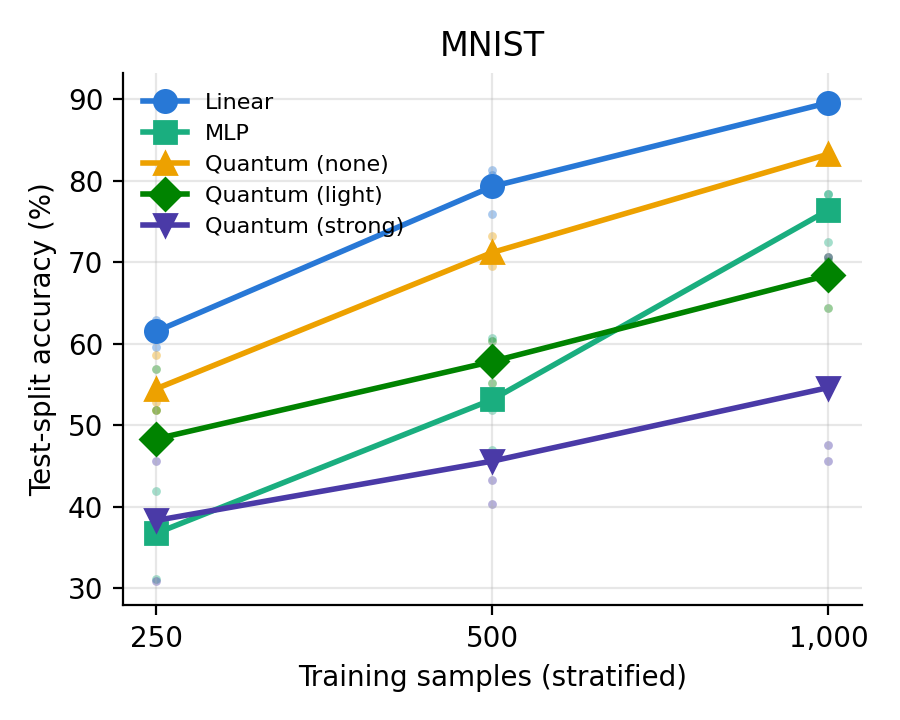
\includegraphics[width=\linewidth]{figures/mnist_accuracy.png}
\end{minipage}\hfill
\begin{minipage}{0.49\textwidth}
  \centering
  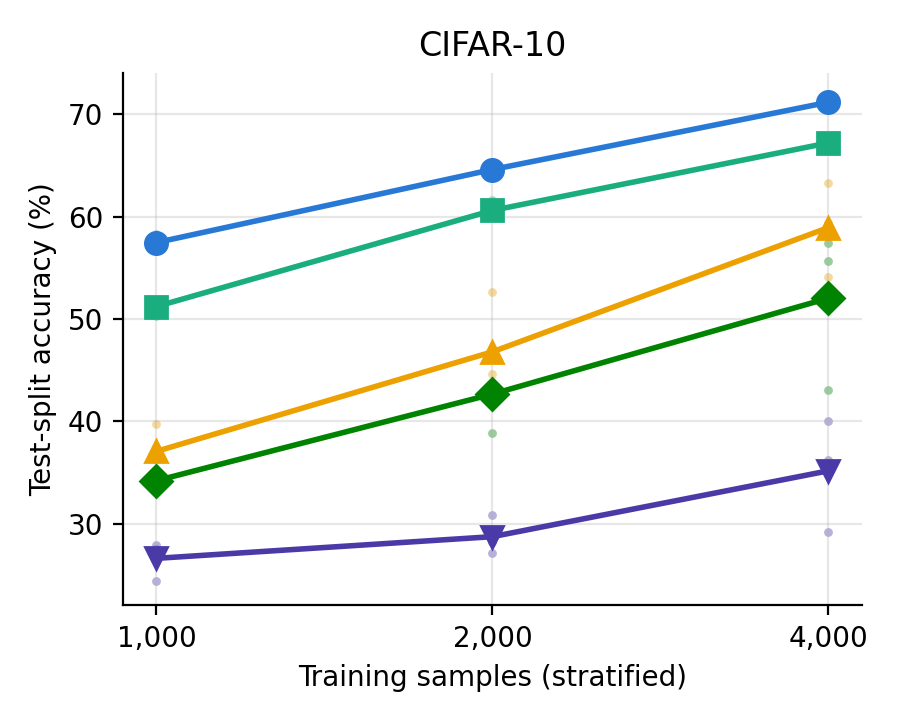
\includegraphics[width=\linewidth]{figures/cifar10_accuracy.png}
\end{minipage}
\caption{Exploratory sweep (shared recipe; Tables~\ref{tab:mnist}--\ref{tab:cifar}):
best test-split accuracy vs.\ stratified training-set size. Solid
lines show the mean over 3 seeds; faint dots show individual seeds. Left:
MNIST. Right: CIFAR-10 (legend shared; note the different vertical scales).
The quantum head (\textsc{none}) sits between the linear and MLP heads on
MNIST but below both on CIFAR-10.}
\label{fig:curves}
\end{figure}

\paragraph{MNIST: under the shared recipe, the quantum head beats the MLP.}
Table~\ref{tab:mnist} shows the VQC head (\textsc{none}) exceeding the
162-parameter MLP by 17.8, 18.0, and 6.9 points at 250, 500, and 1{,}000
training samples, while trailing the 90-parameter linear head by 6--8 points.
Most of this advantage does not survive the protocol of
Section~\ref{sec:protocol}. Moving to that protocol (50 instead of 25 epochs,
validation-based checkpoint selection, the PyTorch simulator) at the same
shared learning rate already reduces it to $+10.8$, $+6.1$ and $-0.5$ points
(paired over seeds). Selecting each head's learning rate on validation then
gives $-2.1$, $+3.3$ and $+0.8$. We cannot separate the effects of the
individual recipe changes.

\paragraph{CIFAR-10: under the shared recipe, the ordering inverts.}
On CIFAR-10 (Table~\ref{tab:cifar}) the VQC head loses to the MLP at every
training-set size, by 14.1, 13.8, and 8.3 points, and to the linear head by
20.4 points at 1{,}000 samples and 12.3 at 4{,}000. This deficit is also
largely recipe-dependent: under the protocol of Section~\ref{sec:protocol},
moving the VQC from the shared learning rate to its validated one gains 6.0,
6.2 and 10.7 points, and its gap to the MLP at 4{,}000 samples falls to 3.1 points
(Section~\ref{sec:protocol}). Accuracy changes little over the final epochs of
these runs, but under a cosine schedule that decays to zero this does not show
convergence, and we do not claim it.

\paragraph{Under the shared recipe, the quantum heads fit their training data poorly.}
We re-evaluated every saved checkpoint in \texttt{eval()} mode on the clean
(unaugmented) training subset and the test split; the per-epoch training
accuracy in the logs is not comparable, being averaged over a changing model on
augmented images in training mode. At 4{,}000 CIFAR-10 samples the clean
train--test gaps are 15.7 (linear), 12.5 (MLP), 8.6 (quantum \textsc{none}) and
1.3 points (quantum \textsc{strong}), with clean training accuracies of 86.9,
79.7, 67.5 and 36.5\%. The strong re-uploading model fits its own training set
barely better than the test set; on MNIST it reaches only 58.5\% clean training
accuracy at 1{,}000 samples. These are statements about what joint training
reached under this recipe, not about representational capacity: at a validated
learning rate the \textsc{none} head reaches 87.9\% clean training accuracy at
4{,}000 CIFAR-10 samples (Section~\ref{sec:protocol}).

\paragraph{The encoding saturates more on CIFAR-10, and saturation tracks seed failures.}
For each quantum checkpoint we measured the fraction of test-split bottleneck
values in the flat region of the encoding, $|\tanh z| > 0.9$. For the
4{,}000-sample \textsc{none} runs it is 16.7, 47.9 and 25.5\% on CIFAR-10
(seeds 0--2) and 4.6, 7.5 and 3.2\% for the 1{,}000-sample MNIST runs. Within
CIFAR-10, saturation and accuracy are strongly anti-correlated across seeds at
fixed training size (Pearson $r=-0.82$ for \textsc{none}, $-0.88$ for
\textsc{light}; 9 runs each): the most saturated seed is the least accurate one
at every size. This is correlational evidence, and it does not explain
re-uploading, whose MNIST checkpoints show essentially no saturation yet still
underperform. Section~\ref{sec:frozen} tests the encoding directly.

\paragraph{Data re-uploading hurts under this recipe.}
Across all six dataset/size conditions, accuracy orders strictly as
\textsc{none} $>$ \textsc{light} $>$ \textsc{strong}. On CIFAR-10 at 2{,}000
samples the strong schedule costs 18.1 points relative to no re-uploading.
We do not have a mechanistic explanation for this. Re-uploading enlarges the
set of frequencies the circuit can access \citep{schuld2021effect}, but that
alone does not determine which functions these fixed circuits can realize, and
we do not distinguish expressivity from trainability here. It contrasts
with the low-dimensional settings where re-uploading is known to help
\citep{perez2020data}. The re-uploading schedules were not included in the
tuned re-run; given how much the \textsc{none} head gains from tuning, this
result should be read as specific to the shared recipe.

\paragraph{Seed variance.}
Classical heads are nearly deterministic across seeds on CIFAR-10 (sample std
$\leq 0.9$ throughout), while quantum heads vary by up to 7.8 points. Given the
correlation above, much of this spread coincides with how saturated the
jointly trained embedding becomes. We do not interpret it as evidence of barren
plateaus \citep{mcclean2018barren}: the circuit is shallow, and the gradient norms we log cover the whole
head including its classical readout, so they cannot diagnose one. Even the best
seed of the best quantum configuration (63.3\%) falls short of the mean
linear-head accuracy on CIFAR-10 (71.2\%). The spread is also
recipe-dependent: under the tuned protocol the \textsc{none} head's sample std
at 4{,}000 CIFAR-10 samples is 1.1 points (4.6 here).

\section{Validation Protocol with Matched Tuning}
\label{sec:protocol}

\paragraph{Protocol.}
For each run we draw a 2{,}000-image validation set, stratified by class, from
the part of the official training set not used for the training subset. The
training subset is the same stratified sample as in the exploratory sweep. The
epoch is selected on validation accuracy. For each (dataset, size, head) cell,
the learning rate with the best mean validation accuracy over seeds
$\{0,1,2\}$ is selected. We report the test accuracy of the selected
checkpoints only; test accuracy for every other grid point is in the released
files. Every head gets the same search: the base learning rate (the backbone
uses half of it, as before) over $\{3\times10^{-4}, 10^{-3}, 3\times10^{-3},
10^{-2}, 3\times10^{-2}\}$ for MNIST and $\{10^{-3}, 3\times10^{-3},
10^{-2}\}$ for CIFAR-10. For every cell whose selected rate was the largest in
the grid, the search was extended by one more step ($10^{-1}$ and
$3\times10^{-2}$ respectively). After this extension the selected rate is
interior for every MLP and VQC cell. The linear head is still at the largest
rate tried on MNIST and at 2{,}000 and 4{,}000 CIFAR-10 samples, so its numbers
may slightly understate the strongest baseline. MNIST runs train for 50 epochs;
CIFAR-10 uses the exploratory recipe (80 epochs, same augmentation). We add the
width-7 MLP (143 parameters), whose stored parameter count is closest to the
VQC's 146 effective parameters. Re-uploading schedules were not re-run.

\begin{table}[t]
\centering
\caption{Test accuracy (\%, mean $\pm$ sample std over 3 seeds) under the
train/validation/test protocol with a matched learning-rate search per head.
Checkpoint epoch and learning rate are selected on validation only. Selected
learning rates: MNIST linear $10^{-1}$; MLP-8 $3\times10^{-2}$; MLP-7
$10^{-2}$, $10^{-2}$, $3\times10^{-2}$; VQC $10^{-2}$. CIFAR-10 linear
$3\times10^{-3}$, $3\times10^{-2}$, $3\times10^{-2}$; MLP $3\times10^{-3}$,
$3\times10^{-3}$, $10^{-2}$; VQC $3\times10^{-3}$, $10^{-2}$, $10^{-2}$.}
\label{tab:protocol}
\small
\begin{tabular}{llcccc}
\toprule
& Train size & Linear (90) & MLP-8 (162) & MLP-7 (143) & VQC (146 eff.) \\
\midrule
\multirow{3}{*}{MNIST}
& 250     & 90.3 $\pm$ 1.9 & 78.7 $\pm$ 6.5 & 75.2 $\pm$ 1.1 & 76.6 $\pm$ 5.3 \\
& 500     & 94.3 $\pm$ 0.2 & 86.7 $\pm$ 3.0 & 87.0 $\pm$ 5.2 & 90.0 $\pm$ 0.6 \\
& 1{,}000 & 96.4 $\pm$ 0.5 & 93.9 $\pm$ 0.8 & 93.7 $\pm$ 0.4 & 94.6 $\pm$ 0.4 \\
\midrule
\multirow{3}{*}{CIFAR-10}
& 1{,}000 & 59.0 $\pm$ 0.9 & 52.3 $\pm$ 1.8 & -- & 43.1 $\pm$ 3.8 \\
& 2{,}000 & 67.6 $\pm$ 0.7 & 62.0 $\pm$ 1.0 & -- & 53.1 $\pm$ 0.9 \\
& 4{,}000 & 74.6 $\pm$ 0.5 & 70.8 $\pm$ 0.5 & -- & 67.7 $\pm$ 1.1 \\
\bottomrule
\end{tabular}
\end{table}

\paragraph{Results.}
Because every head in a cell uses the same seeds, and hence the same training
subset and validation split, we compare heads by paired differences (mean
$\pm$ SD over the three seeds; per-seed values are printed by
\texttt{summarize\_v2.py}). On MNIST, VQC minus MLP-8 is $-2.1 \pm 9.7$,
$+3.3 \pm 2.6$ and $+0.8 \pm 1.0$ points at 250, 500 and 1{,}000 samples, and
VQC minus MLP-7 is $+1.3 \pm 4.6$, $+3.0 \pm 4.9$ and $+0.9 \pm 0.7$. The
17--18-point exploratory advantage is gone. The remaining mean difference is
at most about 3 points; it is positive for every seed only against MLP-8 at 500 samples and
against MLP-7 at 1{,}000. Three seeds cannot establish that the heads are
equivalent, and we do not claim they are. At the shared learning rate of
$10^{-3}$, VQC minus MLP-8 is already $+10.8 \pm 13.9$, $+6.1 \pm 11.6$ and
$-0.5 \pm 3.8$. On MNIST, then, much of the change from Table~\ref{tab:mnist}
comes from the combined protocol changes (epochs and schedule length, checkpoint
selection, simulator), whose individual contributions we do not isolate. The
linear head has the highest mean accuracy in every cell, and among the selected
configurations it beats the VQC for every seed. VQC minus linear is $-13.7$, $-4.3$ and $-1.7$
on MNIST and $-15.8$, $-14.5$ and $-7.0$ on CIFAR-10, negative for every seed.
On CIFAR-10, where the protocol is held fixed and only the learning rate
changes, VQC minus MLP goes from $-13.6 \pm 1.8$, $-13.5 \pm 2.0$ and
$-10.1 \pm 1.6$ at the shared learning rate to $-9.2 \pm 4.5$, $-8.9 \pm 1.7$
and $-3.1 \pm 0.9$ at the selected ones. With tuning the VQC also fits its
training data far better: 87.9\% clean training accuracy at 4{,}000 samples,
versus 67.5\% under the shared recipe. Its under-fitting in
Section~\ref{sec:results} therefore reflects, at least in part, an optimization
setting rather than a fixed limitation. Its accuracy varies by up to 12.4 points
across the CIFAR-10 learning-rate grid (at 2{,}000 samples). Its selected rate
matches both classical heads' at 1{,}000 samples, differs from both at 2{,}000,
and matches only the MLP's at 4{,}000. A head comparison at any single shared
learning rate is therefore unreliable.

\section{Frozen Embeddings: Separating the Head from the Backbone}
\label{sec:frozen}

In joint training each head induces its own backbone, so a head comparison
mixes the two. To separate them we take exploratory-sweep checkpoints of
backbones trained jointly with the linear head and with the VQC head
(\textsc{none}): seeds 0--2, MNIST at 1{,}000 samples and CIFAR-10 at
4{,}000. For each we extract the 8-dimensional embedding once, in
\texttt{eval()} mode on clean images, for three sets: the training subset, a
2{,}000-image validation set drawn as in Section~\ref{sec:protocol}, and the
test split. We then train fresh heads on these fixed embeddings (AdamW, batch
128, 60 epochs, cosine schedule). Epoch and learning rate are selected on
validation. The learning rate is searched in half-decade steps from
$3\times10^{-3}$, and each head's range was extended while its validation
accuracy was still rising at the top. That gives maxima of 10 for the two VQC
heads without a learned affine, 1 for the linear, Fourier and VQC+affine heads,
and 0.3 for the MLP (which diverges at 1) and the 180-epoch VQC. Besides the
linear, MLP and VQC heads we train four more:
\begin{itemize}
  \item a classical \emph{Fourier} head, $[\cos(\pi\tanh z), \sin(\pi\tanh z)]
        \to$ Linear$(16,10)$. It applies the VQC's input nonlinearity without a
        circuit: $\cos(\pi\tanh z_i)$ is exactly $\braket{Z_i}$ after the
        encoding alone.
  \item \emph{VQC+std}: the embedding is standardized with fixed
        training-subset statistics before the unchanged VQC.
  \item \emph{VQC+std+affine}: the same standardization followed by a
        learnable per-dimension scale and shift (16 parameters, initialized
        to the identity).
  \item the VQC trained for 180 instead of 60 epochs (CIFAR-10 only).
\end{itemize}
The source checkpoints were selected on the test split in the exploratory
sweep, so this experiment is itself exploratory, although all selection
within it uses validation only. Because all heads in a column share the same
embeddings, we compare them by paired differences over seeds.

\begin{table}[t]
\centering
\caption{Test accuracy (\%, mean $\pm$ sample std over 3 seeds) of heads
trained on identical frozen embeddings. Columns give the head the backbone was
jointly trained with and, in parentheses, the fraction of test embedding values
with $|\tanh z| > 0.9$. Much of the spread within a column is shared across
heads (it comes from backbone quality), so differences between heads are
reported in the text as paired differences. $^\dagger$Selected learning rate
is the largest tried for that head.}
\label{tab:frozen}
\small
\begin{tabular}{lcccc}
\toprule
& \multicolumn{2}{c}{MNIST (1{,}000 samples)} & \multicolumn{2}{c}{CIFAR-10 (4{,}000 samples)} \\
\cmidrule(lr){2-3}\cmidrule(lr){4-5}
Head & linear src.\ (56\%) & VQC src.\ (5\%) & linear src.\ (66\%) & VQC src.\ (30\%) \\
\midrule
Linear          & 89.8 $\pm$ 0.2 & 88.9 $\pm$ 1.6 & 70.9 $\pm$ 0.6 & 62.5 $\pm$ 4.4$^\dagger$ \\
MLP             & 88.3 $\pm$ 0.9 & 88.5 $\pm$ 1.1 & 70.2 $\pm$ 0.8 & 62.3 $\pm$ 4.0 \\
Fourier         & 78.2 $\pm$ 1.1 & 87.1 $\pm$ 2.0 & 33.4 $\pm$ 1.0 & 61.8 $\pm$ 4.5 \\
VQC             & 69.0 $\pm$ 4.4 & 87.2 $\pm$ 1.0 & 29.1 $\pm$ 3.0 & 61.0 $\pm$ 4.1 \\
VQC+std         & 81.6 $\pm$ 5.6 & 77.6 $\pm$ 6.6 & 59.5 $\pm$ 0.4 & 53.7 $\pm$ 5.6 \\
VQC+std+affine  & 84.0 $\pm$ 3.3 & 82.7 $\pm$ 1.6 & 65.0 $\pm$ 3.1 & 61.6 $\pm$ 4.4 \\
VQC, 3$\times$ epochs & -- & -- & 29.6 $\pm$ 3.0$^\dagger$ & 61.0 $\pm$ 4.5$^\dagger$ \\
\bottomrule
\end{tabular}
\end{table}

\paragraph{On a VQC-trained embedding, the classical heads are slightly better.}
On embeddings from VQC-trained backbones, the linear head beats the VQC head by
$1.7 \pm 0.8$ points on MNIST and $1.6 \pm 0.5$ on CIFAR-10 (paired, mean
$\pm$ SD over seeds). The MLP's margins are
$1.3 \pm 0.1$ and $1.3 \pm 0.4$. The linear and MLP margins are positive for every seed;
they are small, and the marginal standard deviations in Table~\ref{tab:frozen}
hide them because most of that spread is backbone quality. The Fourier head is
level with the VQC on MNIST ($-0.1 \pm 1.1$, mixed in sign) and slightly
ahead on CIFAR-10 ($+0.9 \pm 0.5$). Even on an embedding its
own training shaped, the VQC reads it slightly worse than a linear layer.

\paragraph{The VQC-induced backbone accounts for much of the joint-training gap.}
In the exploratory sweep at 4{,}000 CIFAR-10 samples the jointly trained linear
head beat the jointly trained VQC head by 12.3 points. Two frozen-embedding
contrasts bear on this. A refitted linear head reaches 70.9\% on the
linear-induced embedding but 62.5\% on the VQC-induced one, a backbone contrast
of 8.4 points. On the VQC-induced embedding the refitted linear head beats the
refitted VQC by 1.6 points, a head contrast. Together these account for 9.9 of
the 12.3 points. The remaining 2.3 points are associated with refitting heads
on frozen embeddings rather than training them jointly, so this is not a
complete decomposition, and the split is reference-dependent. With the VQC as
the common readout instead, the same four cells give a backbone contrast of
$-31.9$ and a head contrast of $+41.8$, because the two readouts interact
strongly with the embedding source. What the data does show is that a common
linear probe scores substantially lower on VQC-trained backbones.

\paragraph{The VQC fails on embeddings whose scale does not match its encoding.}
Linear-trained backbones produce embeddings with large magnitudes: 66\% of
CIFAR-10 test values (56\% on MNIST) lie in the flat region of $\pi\tanh z$.
On these embeddings the VQC collapses. It trails a linear head by
$41.8 \pm 2.9$ points on CIFAR-10 and $20.9 \pm 4.4$ on MNIST, while linear
and MLP heads are unaffected. The classical Fourier head, which shares only the
encoding, collapses almost as far on CIFAR-10. It is $4.3 \pm 2.0$ points above
the VQC there and $9.2 \pm 3.6$ above it on MNIST, so on MNIST the encoding
does not account for all of the VQC's loss. Rescaling the input largely repairs
the failure. Fixed standardization alone recovers $30.4 \pm 2.9$ of the 41.8
CIFAR-10 points and $12.6 \pm 6.2$ of 20.9 on MNIST. Adding the learned affine
recovers $35.9 \pm 0.9$ and $15.0 \pm 7.6$, so most of the recovery is ordinary
preprocessing, and learning the scale adds about 5 points on CIFAR-10. Tripling
the training budget recovers $0.5 \pm 0.2$. The direction reverses on
VQC-trained embeddings, which joint training has already fitted to the
encoding (5\% and 30\% saturated). There, fixed standardization \emph{costs}
$9.6 \pm 7.3$ (MNIST) and $7.2 \pm 4.9$ points (CIFAR-10) relative to the
plain VQC. The learned affine undoes this on CIFAR-10 ($+0.6 \pm 0.3$) but only
partly on MNIST ($-4.5 \pm 1.4$). These
results indicate that the VQC is sensitive to the embedding distribution
relative to its fixed encoding, not to normalization as such. They do not
isolate scale from centering. Saturation fraction alone does not predict
accuracy either: standardizing VQC-trained CIFAR-10 embeddings lowers it from
30\% to 12\% yet costs 7.2 points. Neither fixed nor learned rescaling is
uniformly better than leaving a well-matched embedding alone. Only one
longer-training schedule was tested (CIFAR-10 only, at the edge of its
learning-rate grid), so these results show that rescaling beats that
alternative, not that optimization plays no role.

\section{Discussion and Limitations}

\paragraph{Interpretation.}
None of the VQC head's apparent effects in the exploratory sweep survives as an
advantage over a well-run classical head. The large MNIST advantage over the
MLP came from the shared training recipe as a whole: much of it disappears under
the combined protocol changes, and matched learning-rate tuning reduces the
mean difference to at most about 3 points. On CIFAR-10,
where we can hold the protocol fixed, tuning the learning rate alone shrinks the
deficit to the MLP from 10--14 to 3--9 points. In the exploratory checkpoints,
a common linear probe scores 8.4 points lower on VQC-trained backbones than on
linear-trained ones, more than the 1.6 points by which the VQC reads its own
embedding worse than a linear head; this contrast depends on the reference
readout, and we did not repeat it for the tuned runs. On a fixed embedding, the VQC
reads slightly worse than a linear layer when the embedding suits its encoding,
and fails badly when it does not. A classical head with the same $\pi\tanh$
encoding shares much of that failure, and input rescaling largely repairs it.
In every selected configuration, a linear readout is at least as accurate as
the VQC. This matches
the conclusion of broader benchmarks \citep{bowles2024better} in the specific,
widely used setting of a CNN-fed quantum classifier head. For hybrid design it
suggests two things. The distribution of the embedding fed to a fixed-range
angle encoding should be controlled, by training through the encoding or by
rescaling. And quantum heads should be compared against classical heads tuned
on the same budget, ideally on the same embedding.

\paragraph{Limitations.}
This is a bounded empirical study. All quantum results are noiseless
statevector simulations. We study one circuit family ($d=8$ qubits, $L=4$
layers, one encoding), one bottleneck size and two datasets, with three seeds
per cell. That is enough to show consistent signs in paired comparisons, but
not to estimate small effects precisely or to establish equivalence. The tuning
budget covers only the learning rate. The linear head's selected rate is at the
edge of its grid in five of six protocol cells, and some frozen-embedding cells
(marked in Table~\ref{tab:frozen}) are too. Further tuning there could widen
the classical heads' lead, or slightly raise the 180-epoch VQC numbers. Re-uploading schedules were evaluated only
under the shared recipe. The frozen-embedding sources are exploratory
checkpoints selected on the test split, and they cover only two training sizes.
Tables~\ref{tab:mnist}--\ref{tab:cifar} use test-split checkpoint selection and
should be read as exploratory (Section~\ref{sec:methods}). The mechanism claims
concern this circuit and this encoding; whether they extend to other encodings
or deeper circuits is untested.

\section{Conclusion}

Under one shared training recipe, an 8-qubit VQC classifier head appeared to
beat a near-parameter-matched MLP on MNIST by up to 18 points and to lose to it
on CIFAR-10 by up to 14. With longer training, a validation split and the same
learning-rate search for every head, the mean MNIST advantage shrinks to at
most about 3 points and the CIFAR-10 deficit to 3--9 points. On identical frozen
embeddings a linear readout beats the VQC by 1.6--1.7 points when the embedding
suits the encoding. When it does not, the VQC collapses, a classical head with
the same encoding largely shares the failure, and rescaling the input repairs
most of it, while more training recovers little. In every selected configuration a linear readout was at
least as accurate as the VQC. Claims of benefit from small quantum heads in hybrid classifiers should
therefore be made against linear and near-parameter-matched baselines tuned on
the same budget, ideally on a shared embedding.

\paragraph{Reproducibility.}
Code is available at \url{https://github.com/Arkaeyuh/quantcnn}. The
\texttt{results/} directory contains per-epoch metrics and run metadata for
all four completed exploratory sweeps discussed in Section~\ref{sec:methods}, the
checkpoint and frozen-embedding measurements, and the validation-protocol
re-runs; \texttt{scripts/make\_tables.py}, \texttt{analyze\_checkpoints.py},
\texttt{frozen\_heads.py}, \texttt{summarize\_v2.py} and
\texttt{make\_figures.py} regenerate every number and figure in the paper from
those files. The frozen-embedding experiment can be rerun from scratch: the 12
backbone checkpoints it starts from are released in
\texttt{results/frozen\_sources}. Rerunning the clean-image checkpoint analysis
(Section~\ref{sec:results}) needs the other
exploratory checkpoints, which are not released; its outputs are. The batched PyTorch statevector simulator
used for the new experiments is tested against PennyLane to $10^{-6}$ in outputs
and gradients (\texttt{tests/test\_torch\_vqc.py}). Experiments used Python 3.14,
PyTorch 2.11, and PennyLane 0.44 (\texttt{lightning.qubit}, adjoint
differentiation) on an Apple M3 Max; quantum circuits were simulated on CPU
with classical components on the MPS backend. Seeds $\{0, 1, 2\}$ control
Python, NumPy, and PyTorch RNGs as well as subset selection.

\begin{thebibliography}{9}
\small

\bibitem{benedetti2019parameterized}
M.~Benedetti, E.~Lloyd, S.~Sack, and M.~Fiorentini.
\newblock Parameterized quantum circuits as machine learning models.
\newblock \emph{Quantum Science and Technology}, 4(4):043001, 2019.

\bibitem{cerezo2021variational}
M.~Cerezo, A.~Arrasmith, R.~Babbush, S.~C. Benjamin, S.~Endo, K.~Fujii,
J.~R. McClean, K.~Mitarai, X.~Yuan, L.~Cincio, and P.~J. Coles.
\newblock Variational quantum algorithms.
\newblock \emph{Nature Reviews Physics}, 3:625--644, 2021.

\bibitem{mitarai2018quantum}
K.~Mitarai, M.~Negoro, M.~Kitagawa, and K.~Fujii.
\newblock Quantum circuit learning.
\newblock \emph{Physical Review A}, 98:032309, 2018.

\bibitem{havlicek2019supervised}
V.~Havl\'{i}\v{c}ek, A.~D. C\'{o}rcoles, K.~Temme, A.~W. Harrow, A.~Kandala,
J.~M. Chow, and J.~M. Gambetta.
\newblock Supervised learning with quantum-enhanced feature spaces.
\newblock \emph{Nature}, 567:209--212, 2019.

\bibitem{perez2020data}
A.~P\'{e}rez-Salinas, A.~Cervera-Lierta, E.~Gil-Fuster, and J.~I. Latorre.
\newblock Data re-uploading for a universal quantum classifier.
\newblock \emph{Quantum}, 4:226, 2020.

\bibitem{schuld2021effect}
M.~Schuld, R.~Sweke, and J.~J. Meyer.
\newblock Effect of data encoding on the expressive power of variational
quantum-machine-learning models.
\newblock \emph{Physical Review A}, 103:032430, 2021.

\bibitem{mcclean2018barren}
J.~R. McClean, S.~Boixo, V.~N. Smelyanskiy, R.~Babbush, and H.~Neven.
\newblock Barren plateaus in quantum neural network training landscapes.
\newblock \emph{Nature Communications}, 9:4812, 2018.

\bibitem{bowles2024better}
J.~Bowles, S.~Ahmed, and M.~Schuld.
\newblock Better than classical? {T}he subtle art of benchmarking quantum
machine learning models.
\newblock \emph{arXiv:2403.07059}, 2024.

\bibitem{bergholm2018pennylane}
V.~Bergholm et al.
\newblock PennyLane: Automatic differentiation of hybrid quantum-classical
computations.
\newblock \emph{arXiv:1811.04968}, 2018.

\end{thebibliography}

\end{document}
